
\documentclass{article}

%%%%%%%%%%%%%%% LIBRERIAS %%%%%%%%%%%%%%%%%%%%%
\usepackage{amsmath}
\usepackage{titlesec}
\usepackage{titletoc}
\usepackage{graphicx}
\usepackage[spanish,es-tabla]{babel} % 'es-tabla' cambia Cuadro→Tabla
\usepackage{hyperref}                % cargar después de babel



%%%%%%%%%%%%%%%%%%% VARIABLES %%%%%%%%%%%%%%%%%%%%
\newcommand{\Facultad}{Instituto Tecnológico \\de\\ Buenos Aires} %constantes
\newcommand{\TPn}{Trabajo Práctico N° 1}
\newcommand{\TPtema}{Corriente Continua}
\renewcommand{\thesection}{\arabic{section}}          % 2
\renewcommand{\thesubsection}{\quad \alph{subsection}}   % a
\renewcommand{\thesubsubsection}{\quad \thesubsection.~\roman{subsubsection}} % a. i

%%%%%%%%%%%%%%%%%% FORMATO TíTULO %%%%%%%%%%%%%%%%%%%
\titleformat{\section} %formato secciónn
  {\Huge \bfseries}   % formato aplicado al número + título
  {\thesection}      % cómo mostrar el número
  {1em}              % espacio entre número y título
  {}


\titleformat{\subsection} % formato de subsección
{\LARGE \bfseries}
{\thesubsection}
{1em}
{}

\titleformat{\subsubsection} %formato subsubsección
{\large \bfseries}
{\thesubsubsection}
{1em}
{}




%%%%%%%%%%%%%%%%%%% ARCHIVO %%%%%%%%%%%%%%%%%%%%%%%%
\begin{document}

    %%%CARATULA%%%
    \begin{titlepage} %creo portada

        \begin{flushleft}
            \centering
            
\includegraphics[width=0.3\textwidth]{Logo_ITBA.png}
        \end{flushleft}

        \centering
            
        {\scshape\LARGE \Facultad \par} %\par sirve para indicar un final de parrafo
        \vspace{1cm}                    %esto hace un espacio entre lineas de 1cm


        {\huge\bfseries \TPn \par}
        \vspace{1.5cm}
        {\Large Teoría de Circuitos I\\ 25.10 \par}
        \vfill                      %sirve para rellenar el espacio y quede simétrico. Si se añaden otros, se dividen el espacio de forma equitativa
        {\Large \bfseries Grupo N° 5 \par}
        \vspace{1cm}
        {\large Juan Bautista Correa Uranga \hfill Legajo: 65016 \par} %\hfill sirve para hacerlo simétrico
        {\large Juan Ignacio Caorsi \hfill Legajo: 65532  \par}
        {\large Rita Moschini \hfill Legajo: 67026 \par} 
        \vfill
        {\large \today\par}
        \vfil

    \end{titlepage}


    %%%RESUMEN%%%
    {\centering \LARGE \bfseries Resumen \par}
        Aca va el resumen del tp. \par
    \newpage

    %%%INDICE%%%
    \tableofcontents %esto sirve para crear el índice
    \newpage

    %%%Introduccion%%%
    \section{Introducción}

    %%%Desarrollo%%%
    \indent
    \section{Desarrollo}
        \quad Para el desarrollo de este trabajo, se consideró el circuito indicado en la esquemática \autoref{fig:esquemática}.\par
        Para construirlo se usaron los siguientes materiales:\par
        
            	\begin{itemize}
                \item $V_{S_{1}}$ = 12 V
                \item $V_{S_{2}}$ = 5 V
                \item $R_{1} = R_{2} = 220 ~\Omega $
                \item $R_{3} = 680~ \Omega $
                \item $R_{4} = 100~ \Omega $
                \item Resistencia variable con $R_{L_{max}} = 500~\Omega$
                \item Protoboard y cables puentes
                \end{itemize}
        
        
        Primero, se procedió a la construcción del circuito según lo indicado por la esquemática \autoref{fig:esquemática}.\par %falta añadir foto

\begin{figure}[!h]
  \centering
  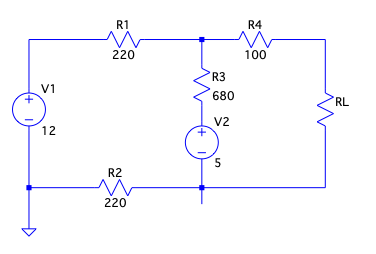
\includegraphics[width=0.5\textwidth]{lab1.png}
  \caption{Esquemática del circuito}
  \label{fig:esquemática}
\end{figure}
        
       Como elementos de medición y alimentación se usaron los siguientes materiales:\par
       
                   \begin{itemize}
                \item Multímetro: UNI-T,  Standar Digital multimiter, modelo: UT39C
                \item Osciloscopio: KEYSIGHT, Digital Storage Osciloscope, modelo: DSOX 1202G 
                \item Fuente DC doble: GW, modelo: GPC-3030D
                \end{itemize}

        Finalmente se midieron con el multímetro los siguientes valores para compararlos con los teoricos. \autoref{tab:resistencias}\par
        
        \begin{table}[h!]
            \centering
            \begin{tabular}{|l|c|c|}
            \hline
            Ri & \multicolumn{1}{l|}{Nominales} & \multicolumn{1}{l|}{Valores medidos} \\ \hline
            R1 & 200  $ \Omega $       & 223     $ \Omega $       \\ \hline
            R2 & 220  $ \Omega $       & 219 $ \Omega $           \\ \hline
            R3 & 680  $ \Omega $       & 667 $ \Omega $           \\ \hline
            R4 & 100  $ \Omega $      & 99 $ \Omega $              \\ \hline
            \end{tabular}
            \caption{Resistencias: nominales vs. medidos}
            \label{tab:resistencias}
        \end{table}

        \subsection{Medición de corriente de Norton, voltaje de Thevenin y resistencia de Norton/Thevenin}
            \subsubsection{Medición}
                \quad Para la primera parte del trabajo, se procedió a la medición de la resistencia de Thevenin, Corriente de Norton y el Voltaje de Thevenin. Para toda esta sección se desconectó la resistencia variable (RL).\par
                En primer lugar, se midió el voltaje de Thevenin. Esto se realizó conectando el voltímetro en paralelo con el nodo A y el nodo B.\par
                En segundo lugar, se midió la Corriente de Norton. Esto se realizó usando el multímetro en modo amperímetro. Para realizar la medición, este se conectó en serie con los extremos A y B. \par
                Finalmente se midió la resistencia de Norton/Thevenin. Para esto, primero se  pasivaron ambas fuentes de tensión. Esto se consiguió apagando ambas fuentes de tensión y luego cambiándolas por cables, haciendo cortocircuito. Por último, se usó el multímetro en modo óhmetro y se conectaron ambas puntas a los nodos A y B.\par

            \subsubsection{Resultados}

                \quad Para esta primera parte se consiguieron los siguientes valores:
            	\begin{itemize}
                \item $V_{Th}$ = 9,29V
                \item $N_{Nt}$ = 24,6 mA
                \item $R_{Th/Nt} = 388  \Omega $
                \end{itemize}

            \subsubsection{Análisis}
            \quad Los valores teóricos calculados según lo explayado en el anexo A son los siguientes:
            	\begin{itemize}
                \item $V_{Th}$ = 9,25 V
                \item $N_{Nt}$ = 25,19 mA
                \item $R_{Th/Nt} = 367,1436  \Omega $
                \end{itemize}
        
        \subsection{Mediciones de potencia}

            \subsubsection{Medición}

            \quad Para esta parte, se añadió la resistencia variable al circuito. Seguidamente, se conectaron un osciloscopio en paralelo con la resistencia variable ($R_{L}$), para medir el voltaje, y un multímetro en modo amperímetro en serie con el circuito y la resistencia.\par
            Luego de esto, se realizó la medición empezando con el potenciómetro en su mínimo valor de resistencia. Luego de anotar los valores de corriente y voltaje, se siguió repitiendo el proceso aumentando el valor de resistencia del potenciómetro hasta llegar al valor máximo.\par
            

            \subsubsection{Resultados}
            
            \quad Los resultados recolectados fueron los siguientes. Observar \autoref{tab:ValoresMedidos2daParte}

            \begin{table}[h!]
            \centering
                \begin{tabular}{|l|c|c|}
                \hline
                Corriente $[mA]$    & Voltaje [V] & \multicolumn{1}{l|}{\begin{tabular}[c]{@{}l@{}}Resistencia $ [\Omega] $ \\ (calculada teoricamente)\end{tabular}} \\ \hline
                22                  & 0,5   & 22,73                                                                 \\ \hline
                20                  & 1      & 50                                                                          \\ \hline
                19,1                & 1,375  &   71,99                                                               \\ \hline
                18,3                & 2      & 109,29                                                                  \\ \hline
                16,9                & 2,5    & 147,93                                                               \\ \hline
                15,1                & 3      &  198,68                                                               \\ \hline
                13,6                & 3,25   & 238,97                                                              \\ \hline
                12                  & 3,875  & 322,92                                                               \\ \hline
                11,4                & 4,5    & 394,74                                                                \\ \hline
                11,3                & 4,625  & 409,29                                                               \\ \hline
                \end{tabular}
            \caption{Valores medidos de la segunda parte de la práctica.}
            \label{tab:ValoresMedidos2daParte}
            \end{table}

            
            
            \subsubsection{Análisis}
                \quad Los resultados recolectados fueron los siguientes. Observar \autoref{tab:ValoresTeoricos2daParte}

            \begin{table}[h!]
            \centering
                \begin{tabular}{|c|c|c|}
                \hline
                Resistencia  $[\Omega]$     & Potencia [mW]         \\ \hline
                30                          & 16,27                 \\ \hline
                60                          & 28,14                 \\ \hline
                90                          & 36,85                 \\ \hline
                120                         & 43,27                 \\ \hline
                150                         & 47,99                 \\ \hline
                180                         & 51,45                 \\ \hline
                210                         & 53,94                 \\ \hline
                240                         & 55,71                 \\ \hline
                270                         & 56,91                 \\ \hline
                300                         & 57,67                 \\ \hline
                330                         & 58,10                 \\ \hline
                360                         & 58,26                 \\ \hline
                390                         & 58,21                 \\ \hline
                420                         & 58,00                 \\ \hline
                450                         & 57,66                 \\ \hline
                480                         & 57,23                 \\ \hline
                \end{tabular}
            \caption{Valores teóricos (para más información, ver anexo B)}
            \label{tab:ValoresTeoricos2daParte}
            \end{table}


    %%%Conclusiones%%%
    \section{Conclusiones}

    %%%Anexos%%%
    \section{Anexos}

\end{document}